\section{EXPERIMENTS}

In this section, we introduce evaluation metrics and briefly introduce a symmetry-aware version of ZebraPose~\cite{su2022zebrapose} - ZebraPoseSAT, then compare our method with other model-based approaches on the T-LESS~\cite{2017tless} and IC-BIN~\cite{icbin} datasets. These datasets encompass a variety of symmetric objects, while a large synthetic-to-real domain gap exists because of texture mismatch. This makes T-LESS and IC-BIN particularly suitable for evaluating the performance of methods on symmetric objects. Furthermore, we present ablation experiments on various hyperparameters and visualizations to intuitively demonstrate the impact of SymCode.

\subsection{Evaluation Protocol}

The Visible Surface Discrepancy (VSD) evaluates the proportion of visible pixels for which the depth absolute discrepancy falls below a threshold of $\tau=20mm$. We report the recall of correct 6D object poses at $e_{VSD}<0.3$~\cite{pitteri2019object}. We also adhere to the evaluation protocol outlined in the BOP challenge~\cite{hodan2024bop} using three metrics: Visible Surface Discrepancy (VSD), Maximum Symmetry-aware Surface Distance (MSSD), and Maximum Symmetry-aware Projection Distance (MSPD). 

\subsection{ZebraPoseSAT: Alternative Symmetry-aware Solution}
To provide a symmetry-aware version of ZebraPose~\cite{su2022zebrapose} for comparison, we additionally implement ZebraPoseSAT (SAT standing for Symmetry-Aware Training), which utilizes an analytical approach~\cite{pitteri2019object} to map all ground truth poses $\mathbf{T}_i$ to a unique $\mathbf{T}$ based on the Frobenius norm, prior to generating the ZebraPose encoding. 
ZebraPoseSAT emerged as the winner of the Best RGB-Only Method in the BOP 2023 challenge~\cite{hodan2024bop}, providing a strong comparison baseline for SymNet.

% However, a challenge arises from the discontinuity observed in the transformation from $\mathcal{F}(I) \rightarrow T$ (representing the network's inference process from an image to pose) around some rotations. For better understanding, let's consider a simple scenario of two-fold symmetry. If we map a degree value from the range $[180, 360)$ into $[0, 180)$, the resulting images at 1 degree and 179 degrees would appear similar, but their corresponding poses would be significantly different.

\subsection{Comparison to State of the Art}

\begin{sidewaystable}[t]
        \centering
        \caption{
                T-LESS: Object recall for $err_{vsd} < 0.3$ on all Primesense test scenes. The results for the $30$ objects are grouped based on their symmetry type.
        }
        \begin{tabular}{r| c c c c c c c c}
        \toprule
        Method& \multicolumn{2}{c}{AAE \cite{sundermeyer2018implicit}} & Pix2Pose \cite{park2019pix2pose}& EdgeEnhance \cite{wen2020edge}& Pitteri\cite{pitteri2019object} & CosyPose\cite{labbe2020cosypose}& Ours(pbr) & Ours(pbr+real)\\
        \cmidrule(lr){2-3}\cmidrule(lr){4-4}\cmidrule(lr){5-5}\cmidrule(lr){6-6}\cmidrule(lr){7-7}\cmidrule(lr){8-9}
        Detector&\ \ \ \ SSD\ \ \ \ \  &\ Retina\ &\ \ Retina\ \ &\ \ Retina\ \ & Faster-RCNN & Retina & FCOS(pbr) & FCOS(pbr+real)\\
        Symmetry type& RGB & RGB & RGB &RGB& RGB &RGB-D& RGB &RGB \\
        \midrule
        Asymmetry (3)&25.98&16.95&24.73&28.76&36.533&-&66.36&\textbf{69.47}\\
        Continuous (11)&11.90&17.98&36.27&39.05&46.65&-&61.52&\textbf{63.72}\\
        Discrete (16)&14.45&18.86&25.79&32.77&38.47&-&69.51&\textbf{78.02}\\
        \midrule
        Mean&14.67 &18.35 &29.5&34.67&41.27 &62.6&66.27&\textbf{71.92} \\
        \bottomrule
        \end{tabular}
\label{tab:tless_vsd}
\end{sidewaystable}

% \begin{table*}[t]
%         \centering
%         \caption{
%                 T-LESS: Object recall for $err_{vsd} < 0.3$ on all Primesense test scene. The symbol $^*$ denotes continuous symmetry, while $^{**}$ denotes discrete symmetry type. 
%         }
%         \begin{tabular}{r| c c c c c c c c}
%         \toprule
%         Method& \multicolumn{2}{c}{AAE \cite{sundermeyer2018implicit}} & Pix2Pose \cite{park2019pix2pose}& EdgeEnhance \cite{wen2020edge}& Pitteri\cite{pitteri2019object} & CosyPose\cite{labbe2020cosypose}& Ours(pbr) & Ours(pbr+real)\\
%         \cmidrule(lr){2-3}\cmidrule(lr){4-4}\cmidrule(lr){5-5}\cmidrule(lr){6-6}\cmidrule(lr){7-7}\cmidrule(lr){8-9}
%         Detector&\ \ \ \ \ \ SSD\ \ \ \ \ \  &\ \ Retina\ \  &\ \ Retina\ \ &\ \ Retina\ \ & Faster-RCNN & Retina & FCOS(pbr) & FCOS(pbr+real)\\
%         Input type& RGB & RGB & RGB &RGB& RGB &RGB-D& RGB &RGB \\
%         \midrule
%         $^*$1&5.65 &8.87&38.4& 37.01&26.35 &-&\textbf{37.99} &25.26 \\
%         $^*$2&5.46 &13.22&35.3&29.78 &\textbf{56.14} &-&25.38 &36.43 \\
%         $^*$3&7.05 &12.47&40.9&44.42 &\textbf{83.33} &-&44.59 &39.86 \\
%         $^*$4&4.61 &6.56&26.3&26.71 &32.98 &-&\textbf{42.02} &32.86 \\
%         $^{**}$5&36.45 &34.80 &55.2&56.22&44.54 &-&\textbf{86.26} &85.57 \\
%         $^{**}$6&23.15 &20.24 &31.5&47.49&\textbf{98.33} &-&61.90 &90.77 \\
%         $^{**}$7&15.97 &16.21 &1.1&26.88&87.74 &-&73.49 &\textbf{95.25} \\
%         $^{**}$8&10.86 &19.74 &13.1&22.98&17.09 &-&78.31 &\textbf{98.28} \\
%         $^{**}$9&19.59 &36.21 &33.9&33.84&52.54 &-&88.53 &\textbf{89.88} \\
%         $^{**}$10&10.47 &11.55 &45.8&35.79&5.43 &-&74.21 &\textbf{87.70} \\
%         $^{**}$11&4.35 &6.31 &30.7&23.27&27.97 &-&49.21 &\textbf{53.27} \\
%         $^{**}$12&7.80 &8.15 &30.4&26.25&43.08 &-&71.43 &\textbf{81.15} \\
%         $^*$13&3.30 &4.91 &31.0&27.70&48.54 &-&63.49 &\textbf{69.71} \\
%         $^*$14&2.85 &4.61 &19.5&16.76&42.19 &-&69.31 &\textbf{76.98} \\
%         $^*$15&7.90 &26.71&56.1&35.81 &47.10 &-&66.73 &\textbf{85.98} \\
%         $^*$16&13.06 &21.73 &66.5&59.31&42.18 &-&57.89 &\textbf{64.29} \\
%         $^*$17&41.70 &64.84 &37.9&55.20&56.83 &-&90.67 &\textbf{93.38} \\
%         18&47.17 &14.30 &45.3&60.11&19.31 &-&90.01 &\textbf{91.01} \\
%         $^{**}$19&15.95 &22.46 &21.7&7.49&27.53 &-&59.67 &\textbf{70.44} \\
%         $^{**}$20&2.17 &5.27 &1.9&9.83&32.16 &-&40.28 &\textbf{53.10} \\
%         21&19.77 &17.93 &19.4&13.77&41.19 &-&54.56 &\textbf{62.45} \\
%         22&11.01 &18.63 &9.5&12.4&49.10 &-&54.51 &\textbf{54.96} \\
%         $^{**}$23&7.98 &18.63 &30.7&24.19&26.08 &-&67.62 &\textbf{73.21} \\
%         $^*$24&4.74 &4.23 &18.3&37.37&41.34 &-&\textbf{83.73} &81.89 \\
%         $^{**}$25&21.91 &18.76 &9.5&33.98&44.37 &-&57.34 &\textbf{61.01} \\
%         $^{**}$26&10.04 &12.62 &13.9&42.54&23.80 &-&63.99 &\textbf{64.19} \\
%         $^{**}$27&7.42 &21.13 &24.4&28.14&33.78 &-&86.41 &\textbf{90.28} \\
%         $^{**}$28&21.78 &23.07 &43.0&56.06&35.10 &-&66.17 &\textbf{66.52} \\
%         $^{**}$29&15.33 &26.65 &25.8&49.3&15.92 &-&87.40 &\textbf{87.70} \\
%         $^*$30&34.63 &29.58 &28.8&59.43&36.17 &-&\textbf{94.91} &94.25 \\
%         \midrule
%         Mean&14.67 &18.35 &29.5&34.67&41.27 &62.6&66.27 &\textbf{71.92} \\
%         \bottomrule
%         \end{tabular}
% \label{tab:tless_vsd}
% \end{table*}

\textbf{Results on T-LESS.} In \Cref{tab:tless_vsd}, we show a comparison with previous methods on the T-LESS dataset for $e_{VSD}<0.3$ recall. We generate the 2D detections using the FCOS~\cite{fcos} detector. The results demonstrate that SymNet outperforms all other methods, achieving a remarkable $25.0\%$ improvement over the results in RGB setting reported by Pitteri et al.~\cite{pitteri2019object}. It is worth noting that the number of recent works providing a comparison based on this specific metric is limited, as the BOP metric offers a more comprehensive and accurate evaluation pipeline. Pitteri et al.~\cite{pitteri2019object} provide the most recent results of $e_{VSD}<0.3$ recall we could find in an RGB setting. Unfortunately, the Retina detector code is outdated and unable to locate detection results. Therefore, we have included results from CosyPose~\cite{labbe2020cosypose}, which also provides BOP scores and $e_{VSD}<0.3$ recall simultaneously. We provide these results to facilitate comparisons with earlier works. Moreover, we have also included results obtained using real images for training. The performance gap between the models trained solely on synthetic data and those incorporating real images is not substantial. This demonstrates the strong generalization capabilities of our method across synthetic and real-world domains. The objects of T-LESS are grouped in 3 categories based on their symmetry type and we provide the average scores for all objects in each category.

\begin{sidewaystable}[t]
        \centering
        \caption{
                BOP results on dataset T-LESS. The time is the runtime per image averaged over the dataset.
        }
        \begin{tabular}{l c c c c c c c c}
        \toprule
        6D object pose estimation method &Input type&Training type&$AR$&$AR_{VSD}$&$AR_{MSSD}$&$AR_{MSPD}$&Time(s)\\       %表格第一行,&的位置对齐
        \midrule
        CDPNv2~\cite{li2019cdpn}&RGB&pbr&0.407&0.303&0.338&0.579&1.849 \\
        CosyPose~\cite{labbe2020cosypose}&RGB&pbr&0.640&0.571&0.589&0.761&0.493\\
        EPOS~\cite{hodan2020epos}&RGB&pbr&0.467&0.380&0.403&0.619&1.992 \\
        ZebraPose~\cite{su2022zebrapose}&RGB&pbr&0.677&0.597&0.636&0.466&0.25 \\
        ZebraPoseSAT-EffnetB4~\cite{su2022zebrapose}&RGB&pbr&0.723&0.659&\textbf{0.695}&0.817&0.25 \\
        SurfEmb~\cite{haugaard2022surfemb}&RGB&pbr&0.735&\textbf{0.661}&0.686&0.857&9.043 \\
        SymNet(Ours)&RGB&pbr&\textbf{0.736}&0.631&0.693&\textbf{0.883}&\textbf{0.093} \\
        \midrule
        DPODv2~\cite{shugurov2021dpodv2}&RGB-D&pbr&0.699&0.646&0.716&0.736&0.320 \\
        \midrule
        ZebraPose~\cite{su2022zebrapose}&RGB&real+pbr&0.775&0.696&0.740&0.889&0.25 \\
        SymNet(Ours)&RGB&real+pbr&0.767&0.674&0.739&0.883&0.058\\
        \bottomrule
        \end{tabular}
\label{tab:tless_bop}
\end{sidewaystable}


\textbf{Results on BOP Benchmark.} We compare our results to other methods that are fully trained on synthetic data, as shown in \Cref{tab:tless_bop} and \Cref{tab:icbin_bop}. We use the default detections provided by BOP challenge 2023~\cite{hodan2024bop}. Since our method does not rely on a time-consuming pose refinement step and directly obtains the pose for every detection, our runtime is significantly reduced compared to the other methods. Our method achieves excellent results in terms of both accuracy and runtime. Specifically, our results match the accuracy of ZebraposeSAT-EffnetB4 but with a smaller backbone, and only at one third of the runtime. Note that we compare the run-time per object instance. However, it should not significantly increase the run-time if inferring multiple objects through parallelization.

\begin{table}[htbp]
        \centering
        \caption{
                IC-BIN 数据集上的 BOP 评估结果
        }
        \resizebox{\textwidth}{!}{%
        \begin{tabular}{l c c c c c c c c}
        \toprule
        6D 物体位姿估计方法 &输入类型&训练类型&$AR$&$AR_{VSD}$&$AR_{MSSD}$&$AR_{MSPD}$&时间(s)\\
        \midrule
        SurfEmb\cite{haugaard2022surfemb}&RGB&pbr&0.588&0.514&0.573&0.678&21.457 \\
        Pix2Pose\cite{park2019pix2pose}&RGBD&real&0.390&0.411&0.384&0.374&3.696 \\
        \midrule
        CDPN\cite{li2019cdpn}&RGB&real&0.327&0.255&0.280&0.447&1.009\\
        EPOS\cite{hodan2020epos}&RGB&pbr&0.363&0.300&0.323&0.465&5.140\\
        CRT-6D\cite{castro2023crt}&RGB&pbr&0.537&\textbf{0.477}&0.517&0.618&0.120 \\
        ZebraPoseSAT-EffnetB4&RGB&pbr&0.545&0.475&\textbf{0.535}&0.625&0.25 \\
        SymNet(本章)&RGB&pbr&\textbf{0.547}&0.450&0.511&\textbf{0.678}&\textbf{0.088} \\
        \bottomrule
        \end{tabular}
        }
\label{tab:icbin_bop}
\end{table}



\subsection{Ablation Studies}
\begin{table}[ht]
        \centering
        \caption{
                Compare CPR module with PnP module on dataset T-LESS.
        }
        \begin{tabular}{c c c c c c}
        \toprule
        CPR & EPnP & $AR$&$AR_{VSD}$&$AR_{MSSD}$&$AR_{MSPD}$\\
        \midrule
                   & \checkmark & 0.283&0.166&0.190&0.493 \\
        \checkmark &            & 0.736&0.631&0.693&0.883 \\
        \bottomrule
        \end{tabular}
\label{tab:ablation_pnp}
\end{table}

\textbf{Compare with PnP solver.} In \Cref{tab:ablation_pnp}, We compare the performance of our CPR module with that of RANSAC/PnP. To the best of our knowledge, this is the only approach to solving one-to-many correspondence scenarios, as demonstrated in SurfEmb~\cite{haugaard2022surfemb}. We randomly sample a one-to-one match from each one-to-many correspondence. Following ZebraPose, we employ the EPnP algorithm~\cite{EPnP}, using 150 iterations, with all correspondences utilized in a single computation step. We believe that with more parallel processing, like that in SurfEmb, we can achieve higher accuracy using RANSAC/PnP, albeit at the cost of time. The results reveal that using PnP alone is challenging in terms of obtaining accurate correspondences, which are crucial for achieving reliable pose estimation. On the other hand, our CPR module is capable of accurately calculating the final pose in real-time.

\textbf{Compare with ZebraPose.} Due to the limitation of one-to-one correspondence, we initially assumed that ZebraPose would not perform well on symmetrical objects. However, in the BOP benchmark, we observe that ZebraPose achieves a satisfactory average recall score of 0.775, which is higher than our result of 0.767 when trained with real data. We attribute this to the utilization of real images during training. Since most objects are not perfectly symmetrical, the network trained with real data can capture subtle variations and mitigate the symmetry problem. We compare ZebraPose trained on real images with that trained on synthetic images in \Cref{fig:vis_zebrapose_gt_real_pbr_support} to support our claims. The results we can access are specifically for the model with a larger backbone, referred to as ZebraPoseSAT-EffnetB4, which has been trained solely on PBR data. However, the results for the ZebraPose model trained exclusively on PBR data are not publicly available. We performed the experiment ourselves using open-source project code, and the average recall score is $0.677$. In the same setting, our score $0.736$ exhibits improvements in both accuracy and inference time.
\begin{figure}[ht]
        \centerline{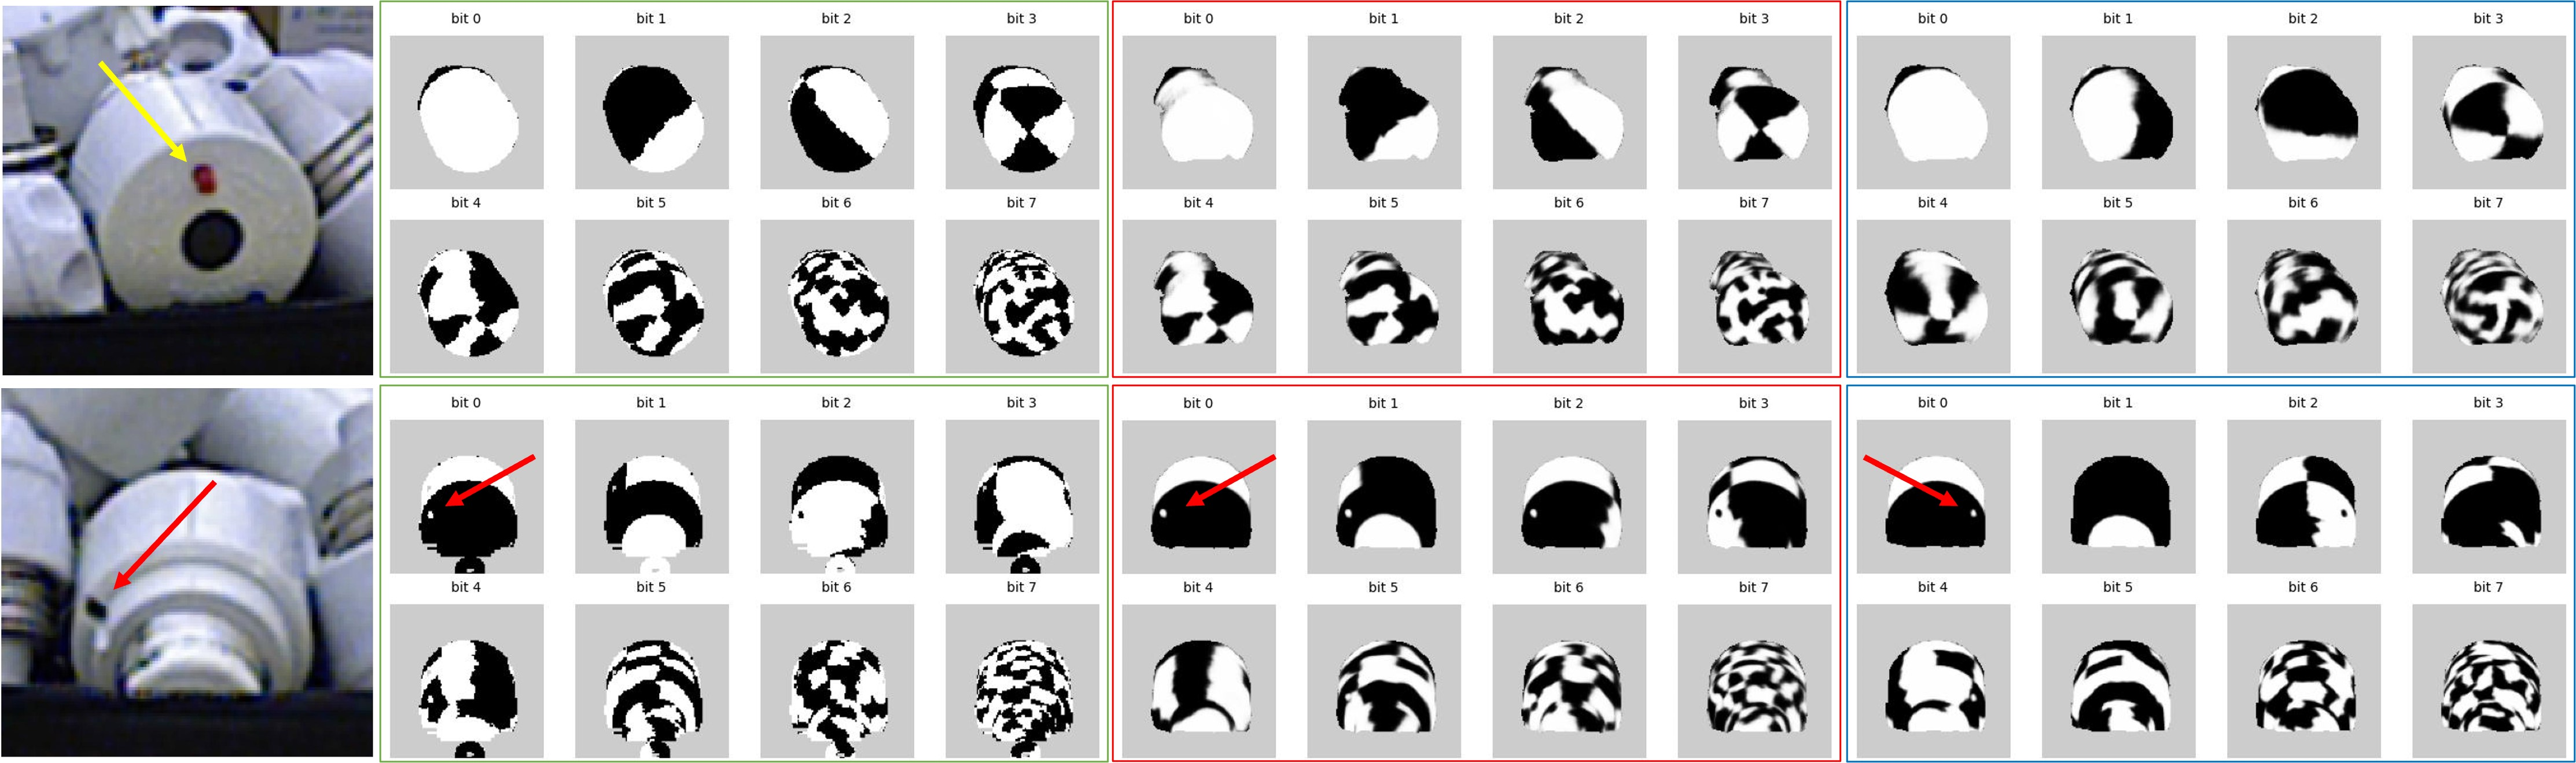
\includegraphics[width=1.0\textwidth]{figure/symnet/vis_zebrapose_gt_real_pbr_support.jpg}}
        \caption{\textbf{ZebraPose(real) vs. ZebraPose(pbr).} Left: input image. \textcolor{green}{The green box} indicates the ground truth, \textcolor{red}{the red box} shows the ZebraPose encoding trained with real data, and \textcolor{blue}{the blue box} represents the ZebraPose encoding trained with synthetic data. We visualize two cases for the T-LESS obj04 object, which features a red section (indicated by the yellow arrow) at the top and two dents (indicated by the red arrows) in the middle, disrupting its continuous symmetry. It can be observed that the results of the model trained on real data are closer to the ground truth, as the network can leverage subtle surface distinctions to avoid ambiguity during training with real images. These subtle distinctions exist in the simulation data but are less pronounced; for instance, color information is absent in the T-LESS synthetic training data.}
        \label{fig:vis_zebrapose_gt_real_pbr_support}
\end{figure}

\textbf{Length of SymCode.} The default setting of length for $d$ is $16$ as used in ZebraPose~\cite{su2022zebrapose}. We investigate the impact of varying $d$ on the training process, as illustrated in~\Cref{fig:ablation_bit}. The results indicate that our approach is robust to variations in the length of the binary code. Indeed, the accuracy achieved with different values of $d$ can be unpredictable, and there is no clear way to determine an optimized value beforehand. As a result, in our main results, we have chosen to fix the length of the binary code to the default value of $16$. As shown in \Cref{fig:compare_gt_est}, the network performs poorly on the last few bits, which can also be observed in ZebraPose. From \Cref{fig:ablation_bit}, it is evident that a length of 16 is the worst choice. This suggests that there is still room for optimization in the length of the code. So we performed comparisons using lengths of 16 and 10 for the add-s metric on YCB-V dataset, with results improving from 73.68 to 74.66. Since this improvement was not substantial, we did not explore other lengths further.
% This ensures consistency in our experiments while avoiding potential biases introduced by selecting different values of it.

\begin{figure}[th]
        \centerline{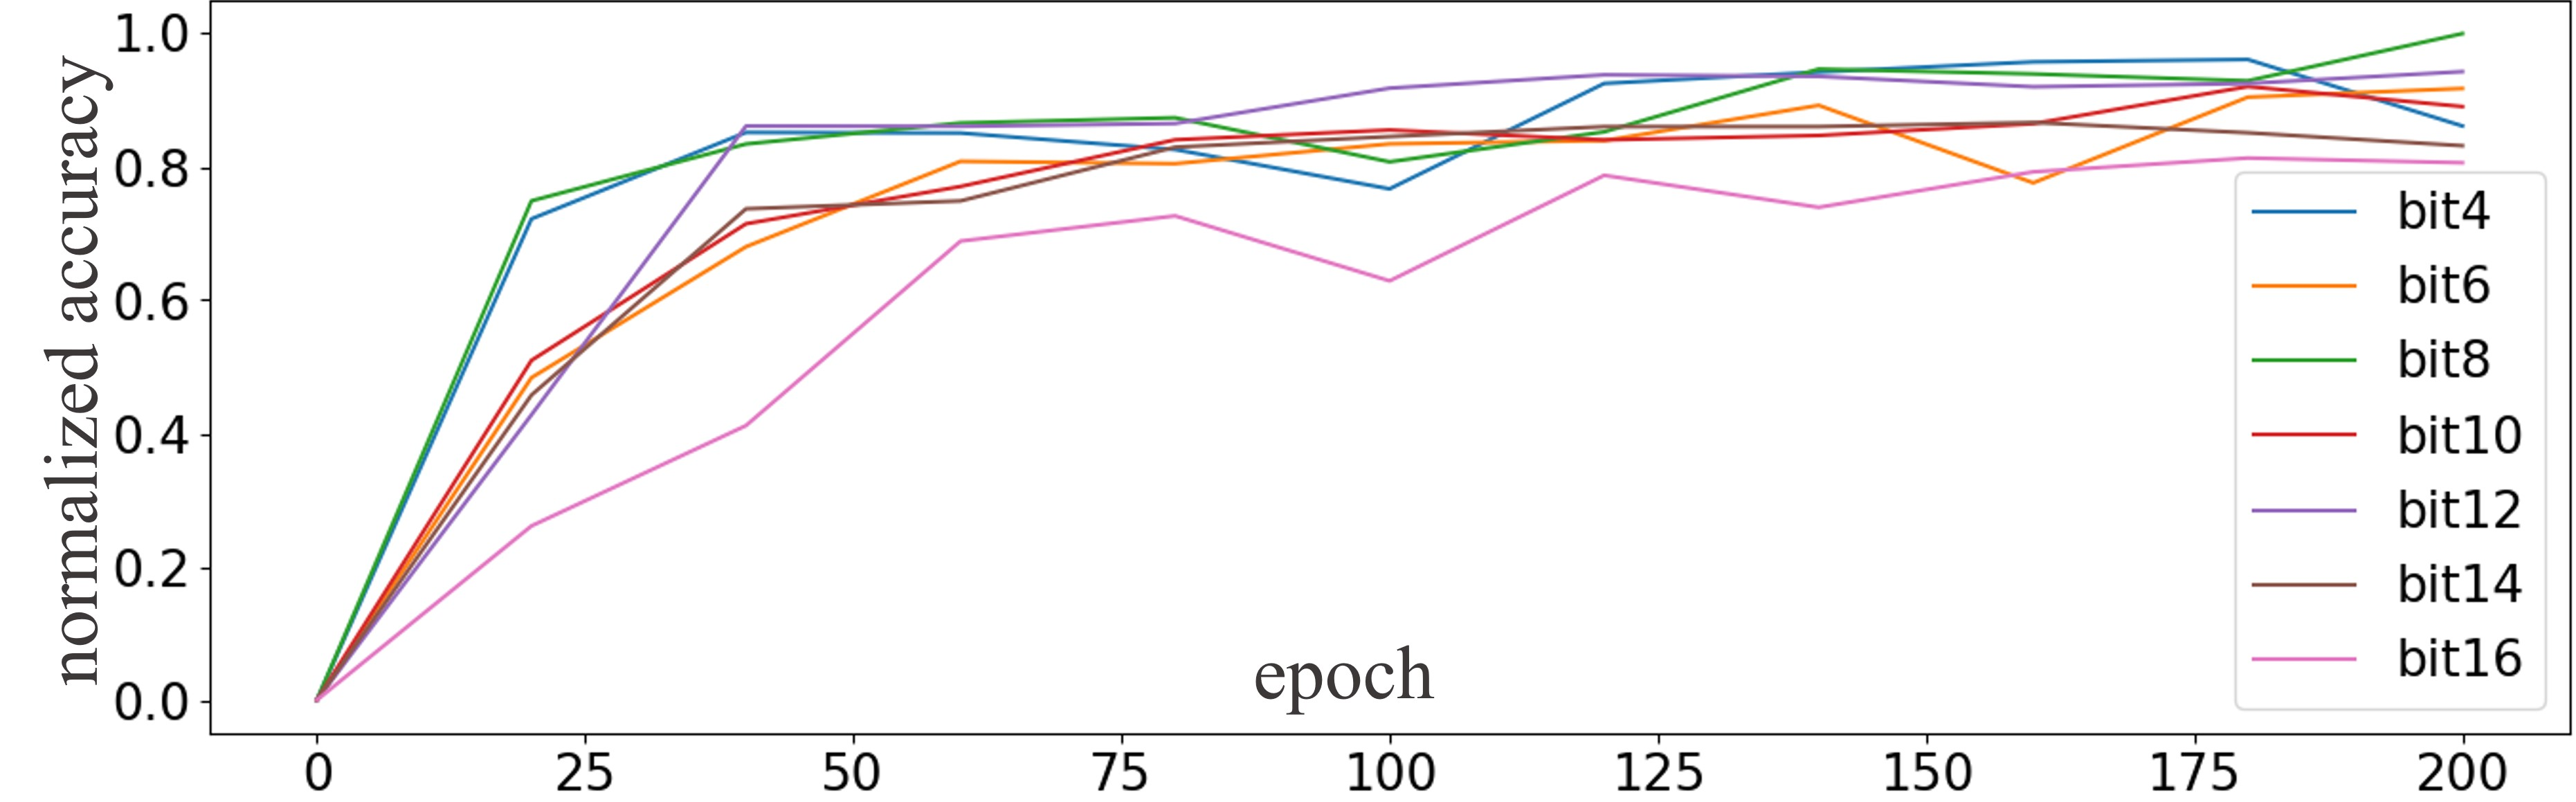
\includegraphics[width=0.85\textwidth]{figure/symnet/ablation_bit.jpg}}
        \caption{We performed an ablation study on object 27 from T-LESS dataset, which exhibits discrete symmetry, to determine the optimal length of the binary code $d$. We normalized the BOP score to represent accuracy. The resulting curve demonstrates that even with a small number of bits (8 bits), our method is capable of capturing the object's pose.}
        \label{fig:ablation_bit}
\end{figure}

\begin{figure}[th]
        \centerline{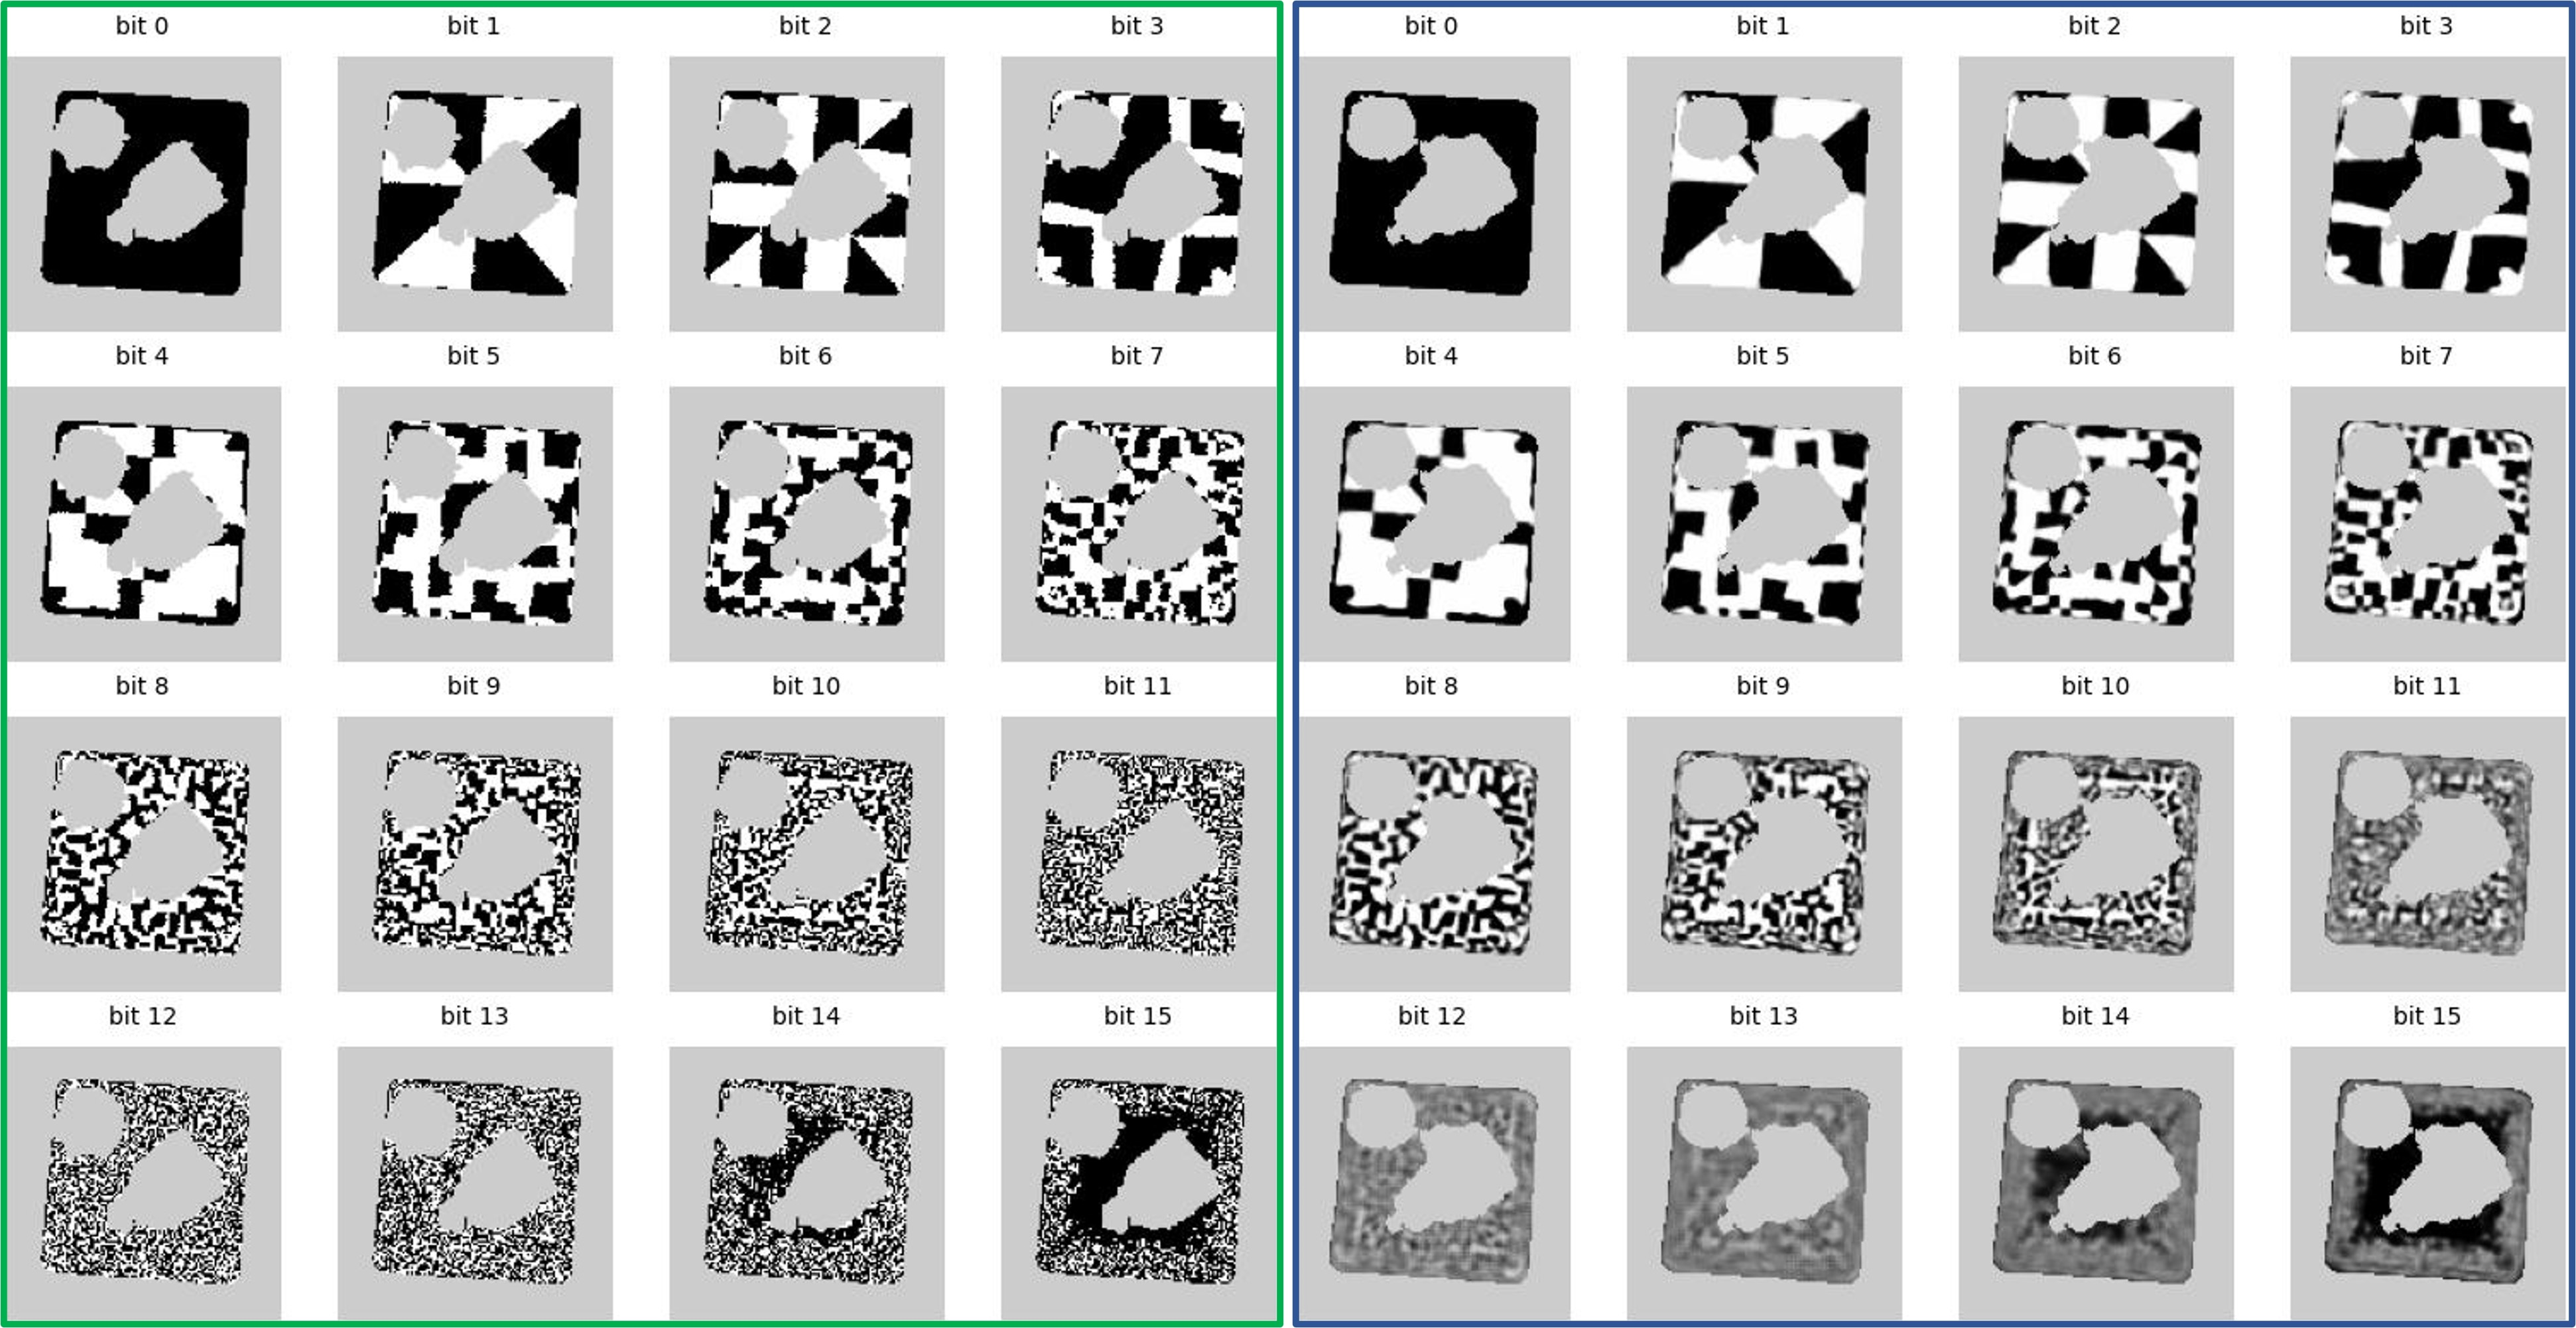
\includegraphics[width=0.85\textwidth]{figure/symnet/compare_gt_est.jpg}}
        \caption{Left: Ground truth of the 16-bit SymCode. Right: Estimated SymCode. This suggests that there is still room for optimization in the length of the code.}
        \label{fig:compare_gt_est}
\end{figure}

\textbf{Challenge of learning one-to-one correspondences.} We conducted experiments involving training our end-to-end network using ZebraPose encodings, which is an efficient way to encode one-to-one correspondences. In this case, the network achieved a BOP recall of 0.612, which is relatively weaker compared to SymNet's performance of 0.736. When we removed all the end-to-end loss and focused solely on training the ZebraPose encodings, \Cref{fig:difficult_learn_one_to_one} illustrates the challenges associated with learning one-to-one correspondence-based encodings.

\begin{figure}[ht]
    \centerline{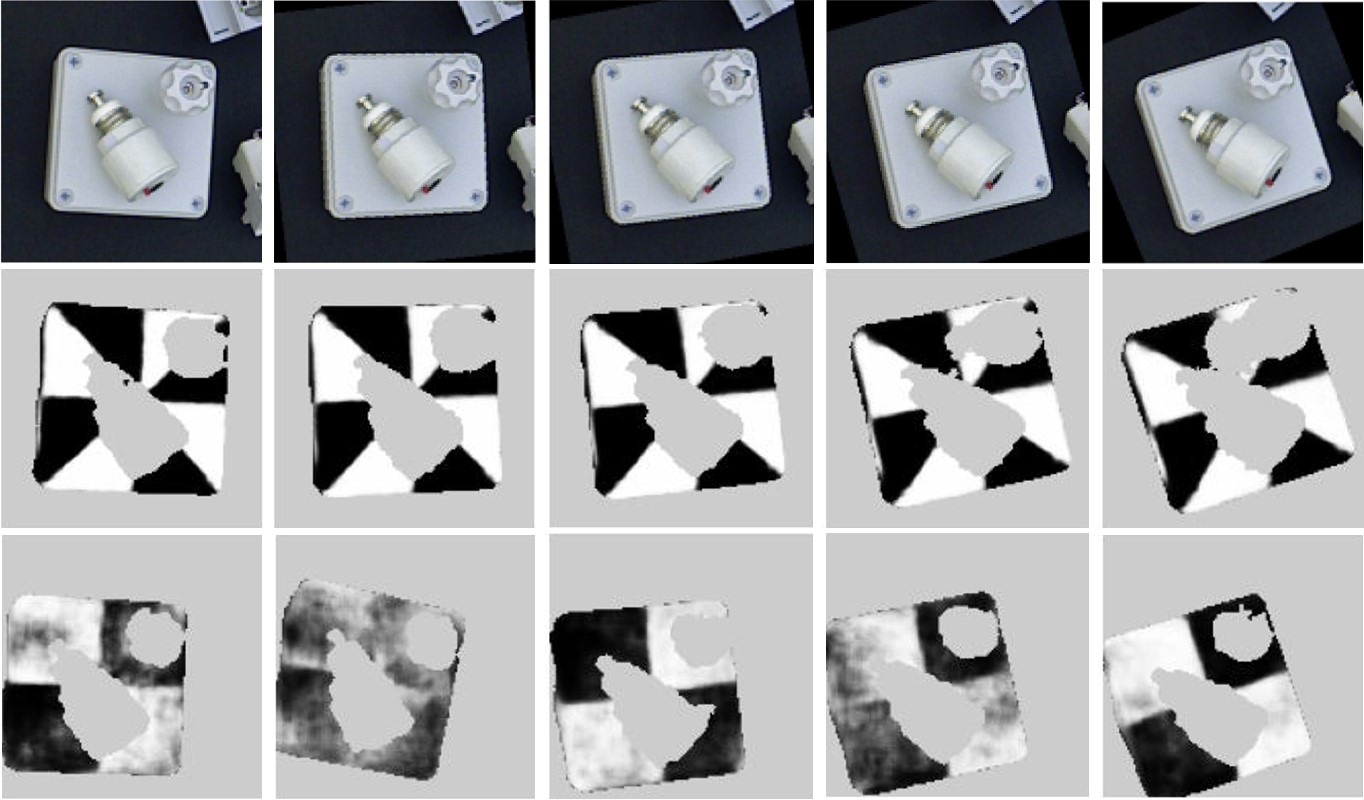
\includegraphics[width=0.85\textwidth]{figure/symnet/difficulty_learn_one_to_one.jpg}}
    \caption{\textbf{The challenge of learning one-to-one correspondences.} First line: The images with similar viewpoints. Second line: the 2nd bit prediction of SymCode. Third line: the 2nd bit prediction of ZebraPose Code. In order to achieve high accuracy pose estimation, ZebraPose Code relies on RANSAC-PnP to filter out inconsistent correspondences. However, there are still cases (second column) where ZebraPose struggles due to the ambiguity arising from symmetries. Please note that the result was obtained using our SymNet network trained with ZebraPose Code. To achieve a clear visualization, we have applied a mask based on the predicted mask to remove the background. In the visualization of the predictions, we have represented a value of 0 as black and a value of 1 as white. Any value between 0 and 1 is displayed as a shade of gray. }
    \label{fig:difficult_learn_one_to_one}
\end{figure}

\begin{figure}[th]
    \centerline{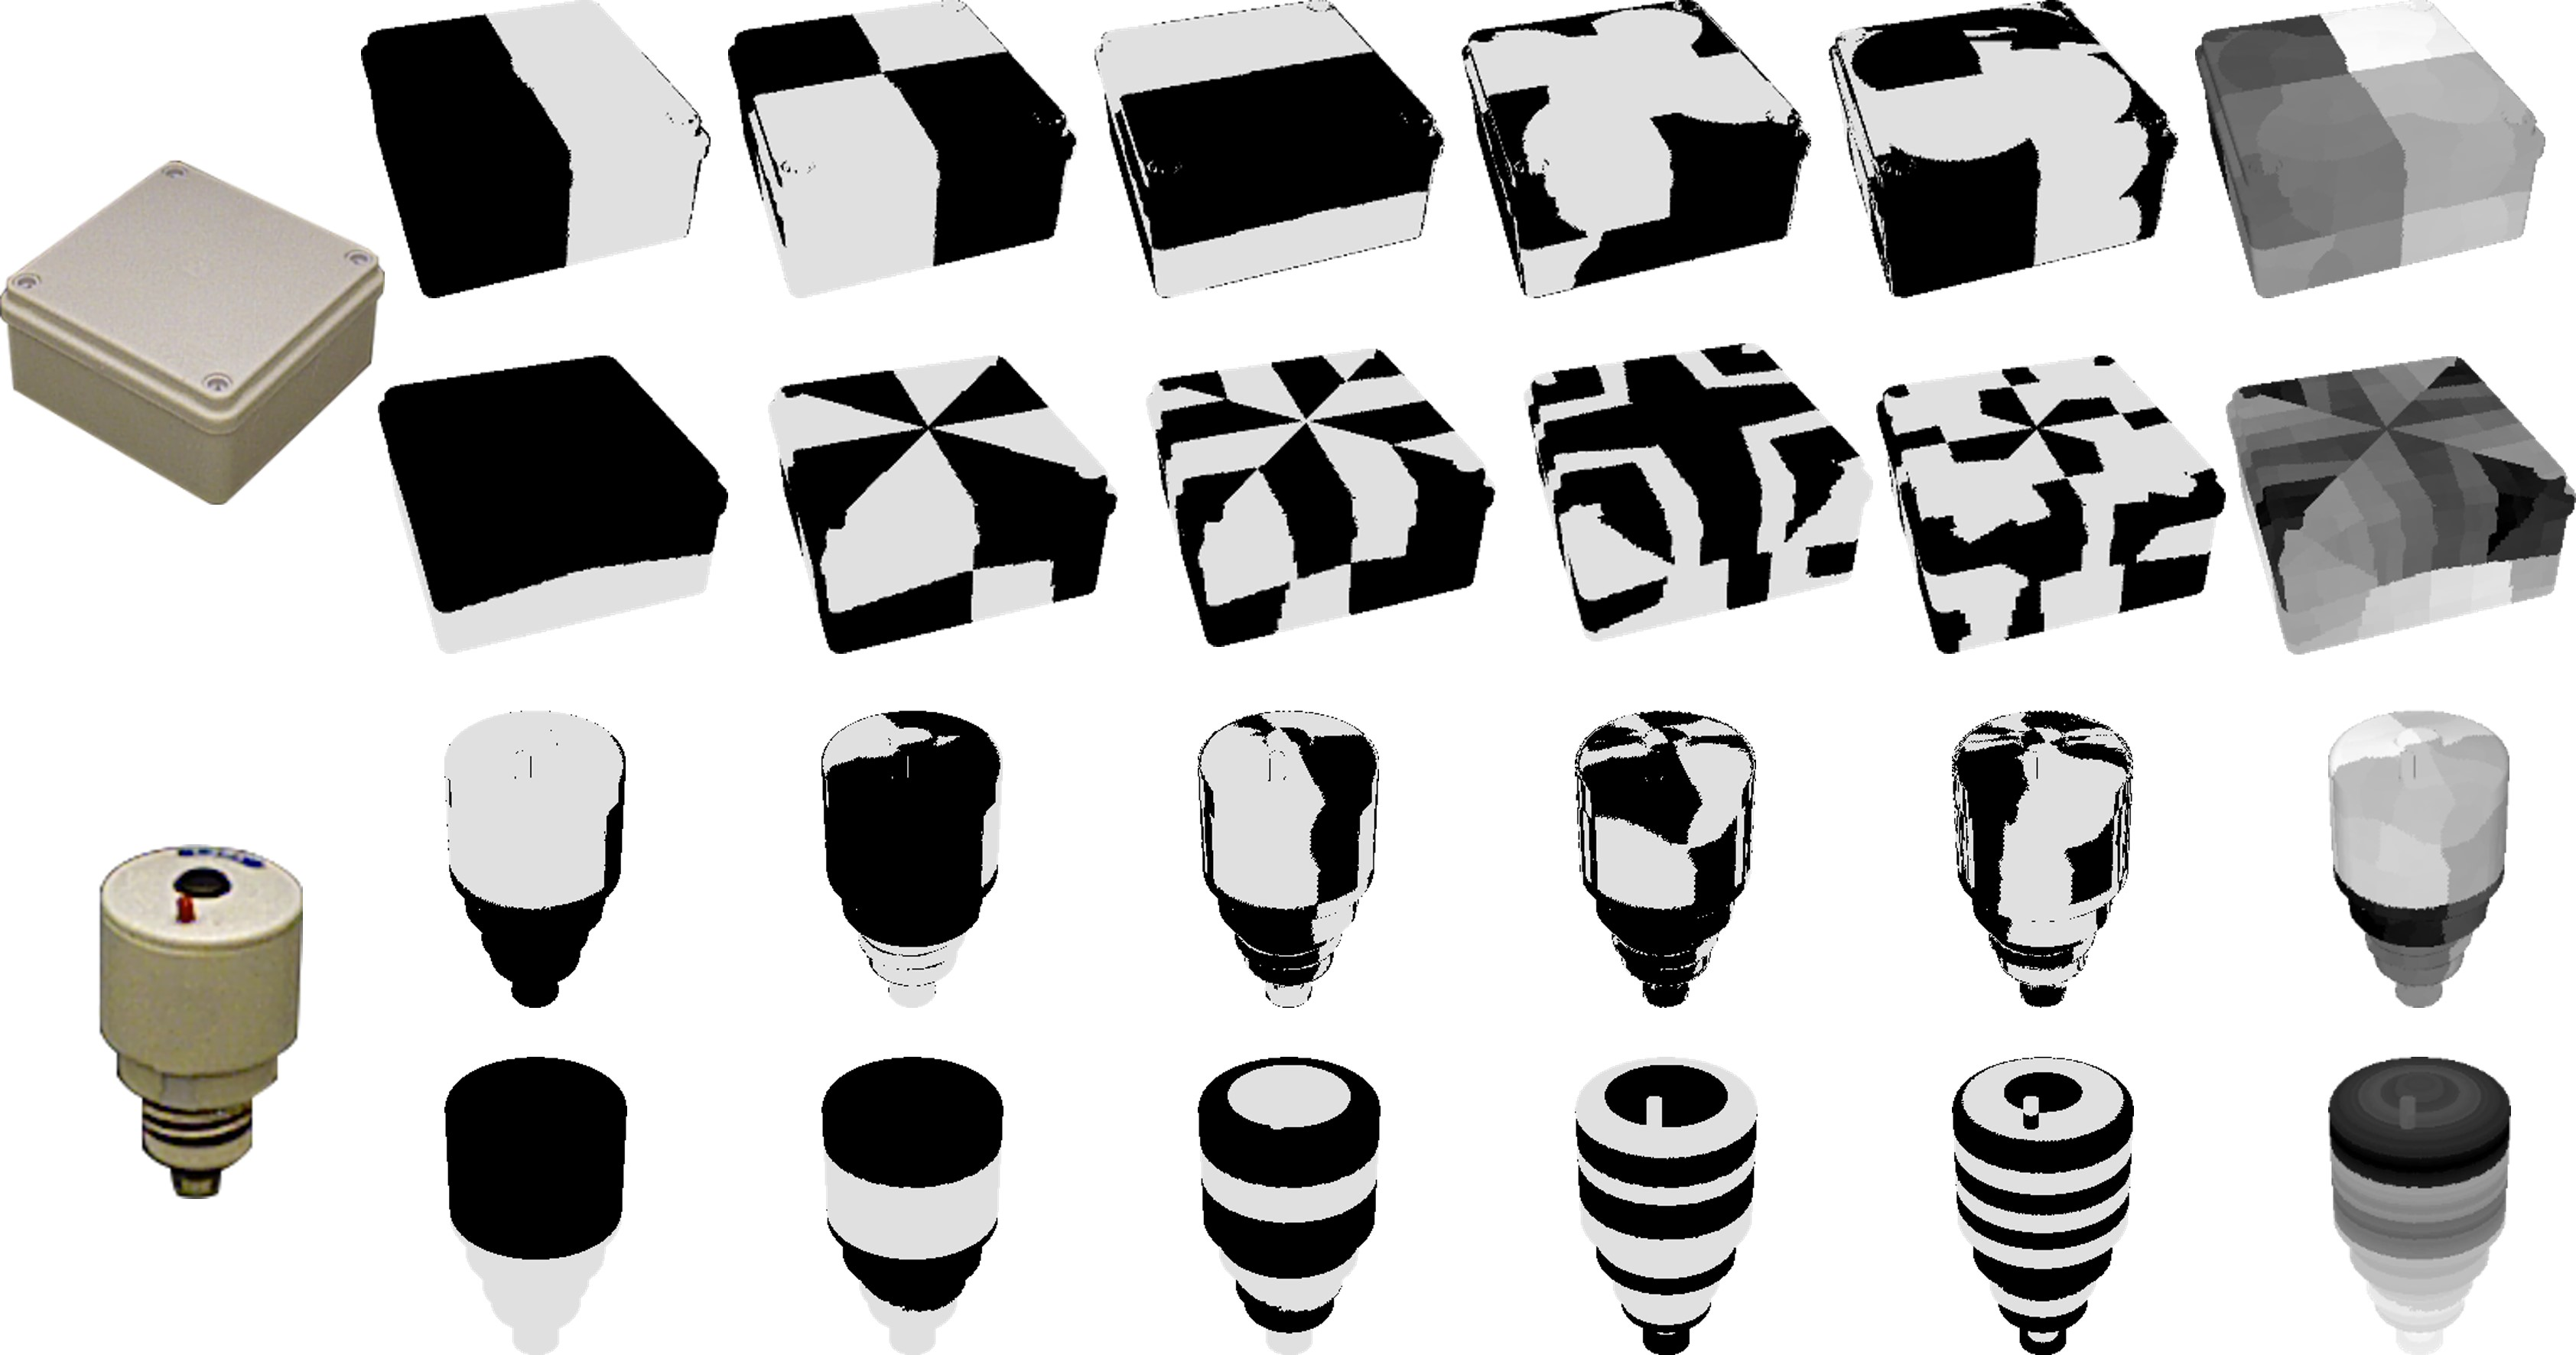
\includegraphics[width=0.85\textwidth]{figure/symnet/compare_code_map.jpg}}
    \caption{\textbf{Comparison of code maps.} Detailed binary code maps representing SymCode and ZebraPose are visualized for two objects. The first and third rows depict the code maps for ZebraPose, while the second and fourth rows illustrate those for SymCode. The final columns aggregate the results for all the bits.}
    \label{fig:compare_code_map}
\end{figure}

\begin{figure}[ht]
    \centerline{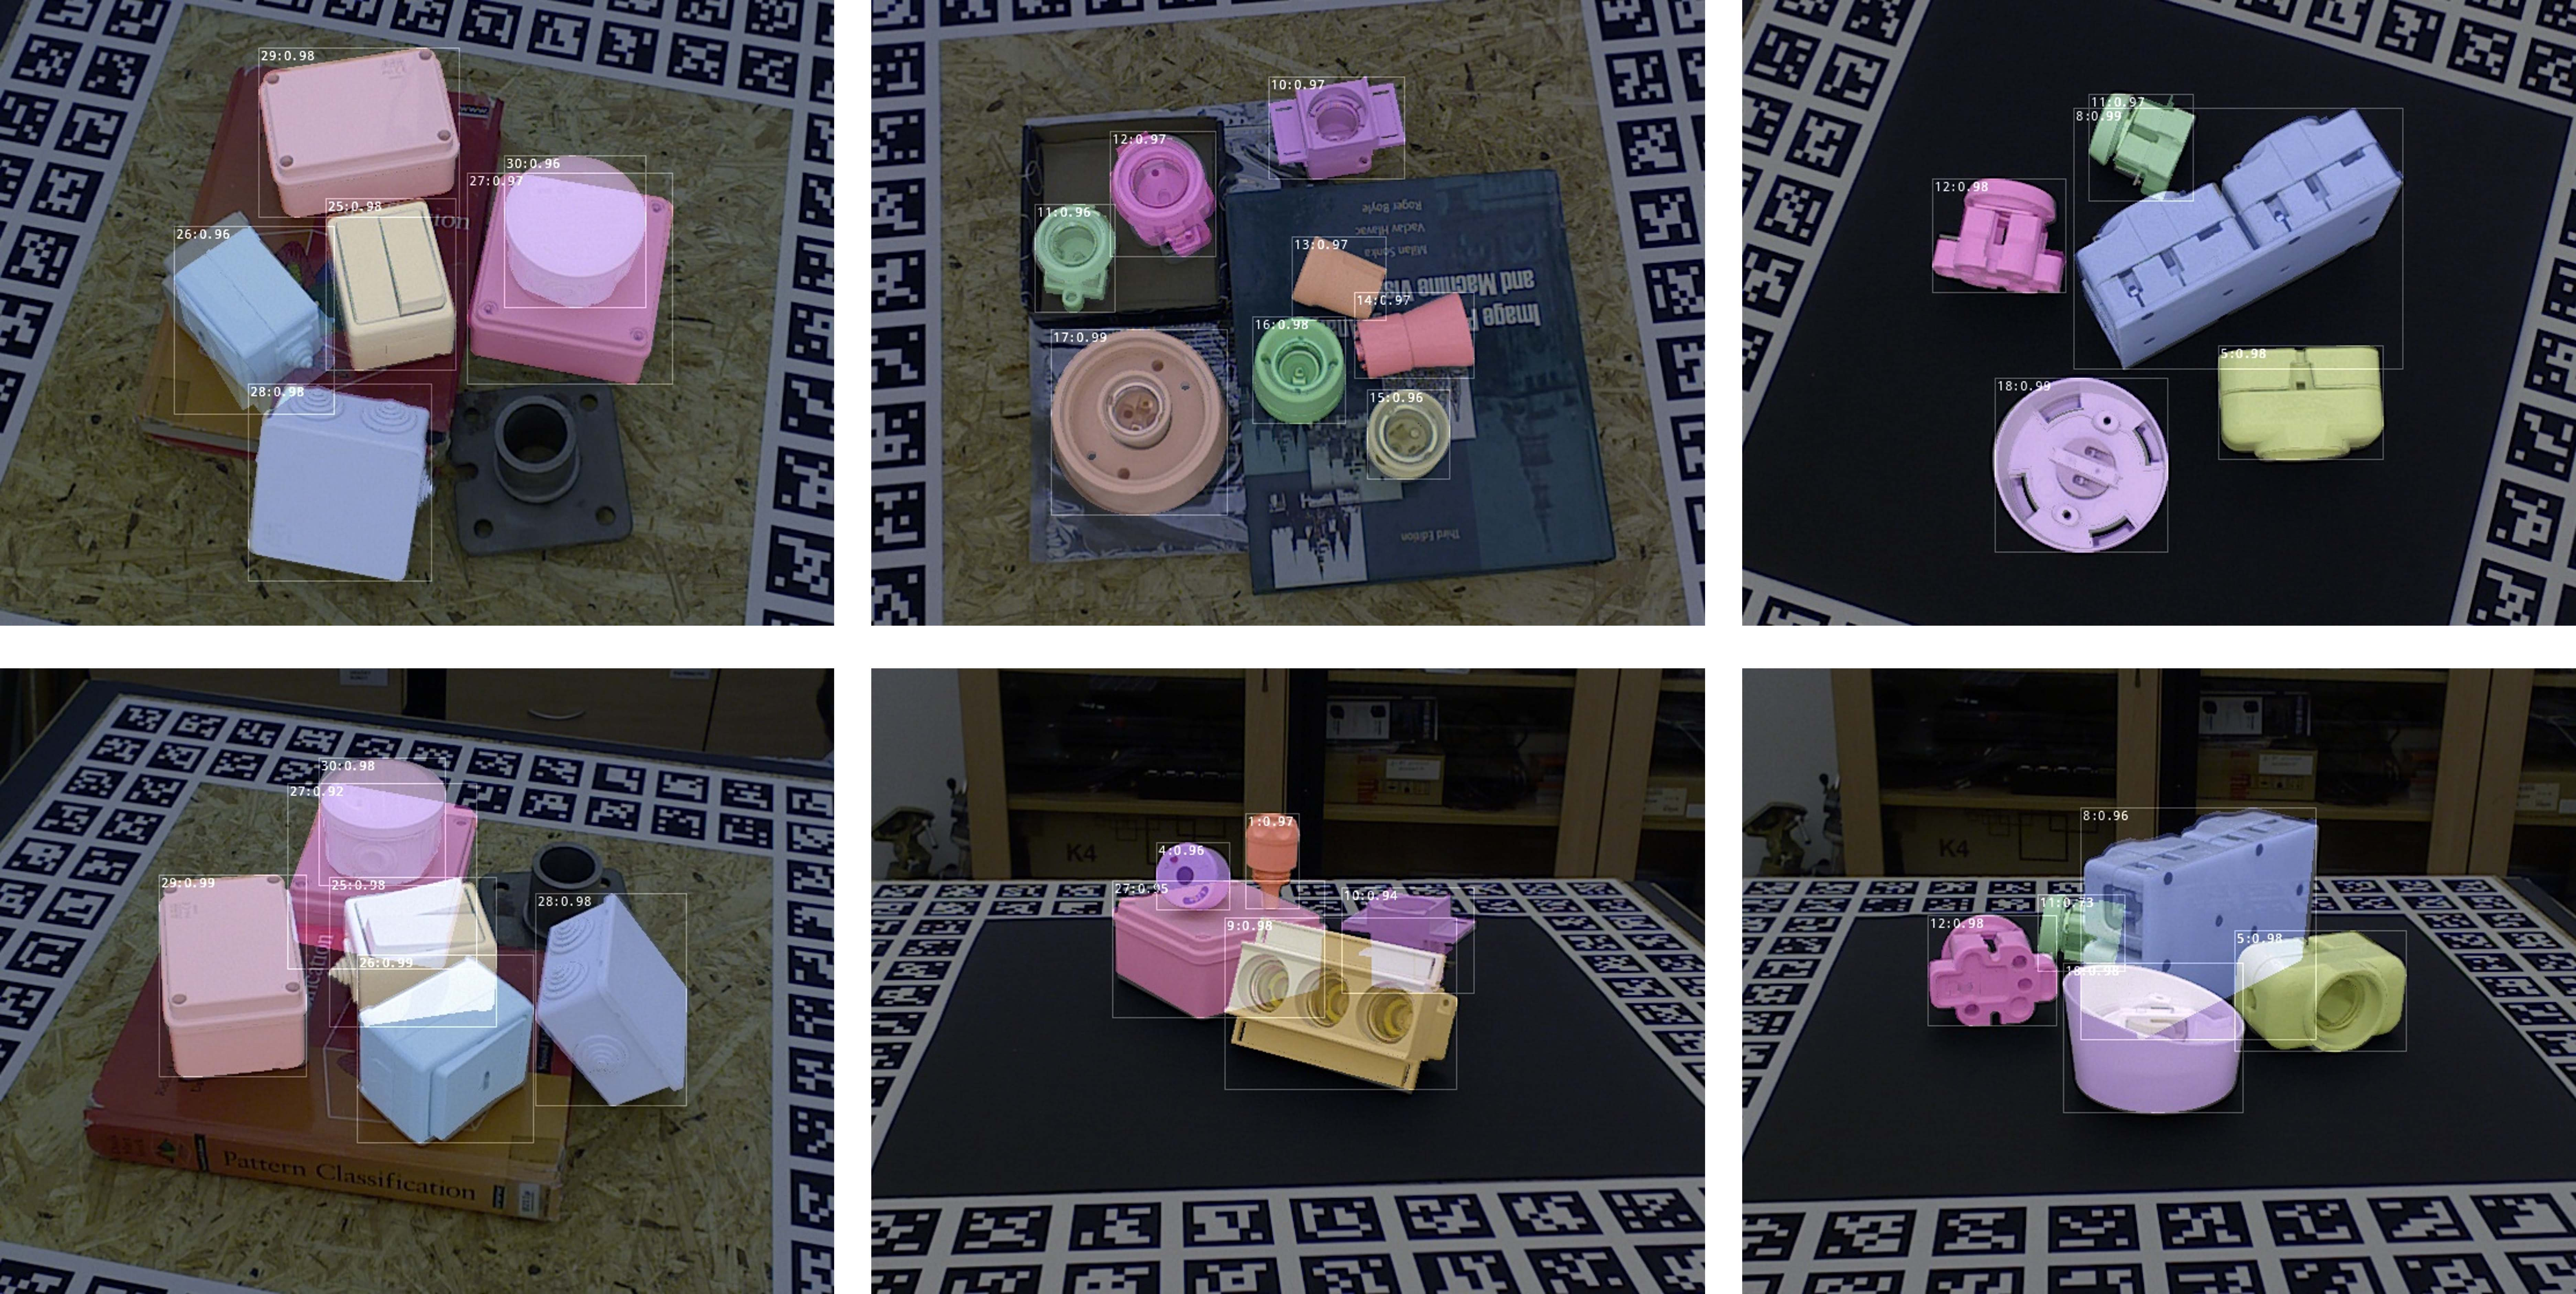
\includegraphics[width=0.85\textwidth]{figure/symnet/visualization_tless.jpg}}
    \caption{\textbf{Qualitative Result on T-LESS~\cite{2017tless}.} We render the objects with the estimated pose on top of the original images. The presented confidence scores are from the 2D object detection provided by BOP challenge 2023~\cite{hodan2024bop}. Each column represents a scene captured from a different viewpoint. The visualizations demonstrate that our method is capable of effectively handling severe occlusion in cluttered  environment.}
    \label{fig:visualization_tless}
\end{figure}

\begin{figure}[th]
        \centerline{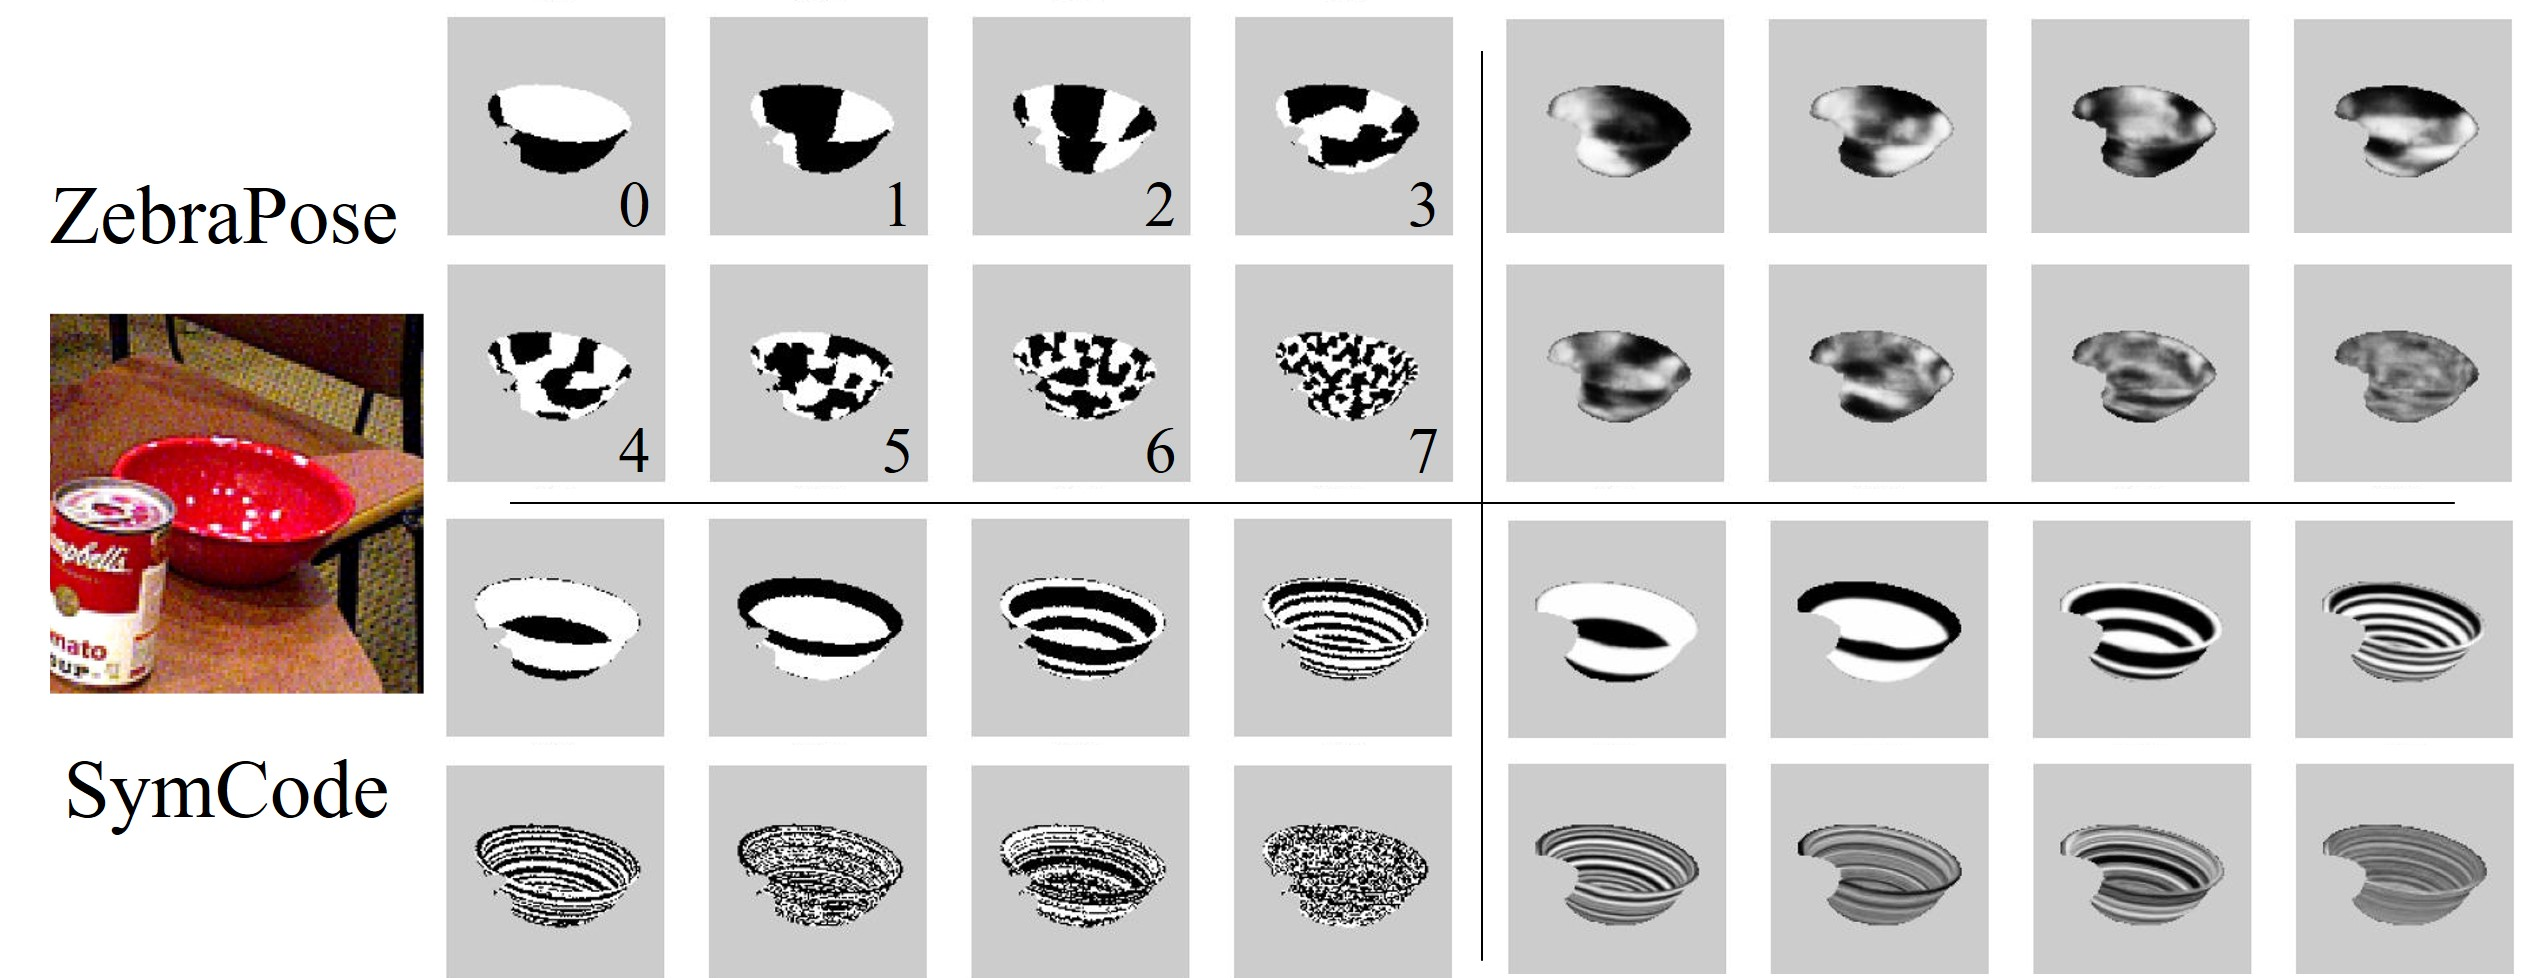
\includegraphics[width=0.85\textwidth]{figure/symnet/compare_with_zebrapose.jpg}}
        \caption{\textbf{Comparison with ZebraPose.} Upper Left: Ground truth of ZebraPose. Upper Right: Predicted output of ZebraPose. Bottom Left: Ground truth of SymCode. Bottom Right: Predicted output of SymCode. Only the first 8 bits are displayed. It appears that SymNet tends to be more confident in its outputs, often producing predictions closer to extreme values of 0 or 1. On the other hand, ZebraPose's predictions tend to be more centered around 0.5, indicating a lower level of confidence.}
        \label{fig:compare_zebrapose}
\end{figure}

\textbf{Visualization.} Detailed binary code maps representing SymNet and ZebraPose are visualized in~\Cref{fig:compare_code_map}, which shows our binary codes contain symmetry information. Qualitative results on T-LESS~\cite{2017tless} can be found in~\Cref{fig:visualization_tless}. A visual representation of the ground truth and predicted code maps for ZebraPose and SymNet is shown in~\Cref{fig:compare_zebrapose}. From the visualization, it is evident that ZebraPose struggles to accurately reproduce the ground truth, whereas SymNet exhibits better performance in this regard.


% In this section, we begin by introducing the implementation details, datasets, and evaluation metrics employed. Following that, we compare the performance of our method with other model-based approaches on the T-LESS dataset~\cite{2017tless}. The T-LESS dataset encompasses a variety of symmetric objects without textures, while a large synthetic-to-real domain gap exists because of texture mismatch. This makes T-LESS particularly suitable for evaluating the performance of methods on symmetric objects. Additionally, we present ablation experiments on different hyperparameters.

% \subsection{Implementation Details}
% The process of surface encoding and label generation is built upon Open3D~\cite{Zhou2018open3d}. By default, the length of the binary code, $d$, is set to be $16$. Our method is specifically designed for each object, as this setting remains crucial for high-precision applications, offering significant advantages compared to training a single model to cover multiple objects.

% The input image is cropped and resized to an RoI with dimensions of $256\times 256\times 3$, based on the detection result. If not explicitly stated, we utilize the bounding box detected by YoloX~\cite{ge2021yolox}. The shape of the intermediate variables is set to be $128 \times 128$. During training, we employed a dynamic zoom-in strategy to generate noisy RoI with varying sizes in the range of $[1.2-1.5]$. However, during inference, the RoI scale rate is fixed at $1.3$. We apply strong augmentations to the input image, similar to the approach used in GDR-Net~\cite{wang2021gdr}, in order to simulate variations in lighting, occlusion, and a clustered environment. The network is trained for a maximum of $300$ epochs using the Adam optimizer~\cite{Kingma2014AdamAM}. We use a batch size of either $16$ or $32$ and a fixed learning rate of $2e-4$. The balancing weight in the loss function is set to a default value of $\alpha = 3$. Our network can be trained on a single NVIDIA 2080Ti GPU.

% \subsection{Datasets}
% We evaluated our method on the T-LESS dataset~\cite{2017tless}.

% The T-LESS dataset consists of 30 industry-relevant objects that lack significant texture or discriminative color. These objects demonstrate symmetrical and morphological similarities, with some being composite structures. They are uniformly white and symmetrical, resembling typical industrial items. The dataset includes test images captured by the Primesense CARMINE 1.09, a structured-light RGB-D sensor, as well as the Microsoft Kinect v2, a time-of-flight RGB-D sensor. Scene complexity ranges from simple setups with a few isolated objects to highly challenging scenarios featuring multiple instances of objects amidst clutter and occlusion. Test images are drawn from 20 scenes, each presenting varying levels of complexity.

% To mitigate the time-consuming process of annotating real data for object pose, we leverage publicly available synthetic physically-based rendered (pbr) images provided by the BOP challenge~\cite{hodan2018bop}. These synthetic images allow us to demonstrate the effectiveness of our network when trained solely on synthetic data.

% \subsection{Evaluation Protocol}

% The Visible Surface Discrepancy (VSD) is a widely used metric that compares ground truth measured depth maps with depth maps rendered based on estimated poses. It evaluates the proportion of visible pixels for which the depth absolute discrepancy falls below a threshold of $\tau=20mm$. Consistent with prior research~\cite{wen2020edge, pitteri2019object}, we report the recall of correct 6D object poses at $e_{VSD}<0.3$. Notably, this metric demonstrates reduced sensitivity to visual symmetries, as they often result in analogous symmetries within depth maps.

% We adhere to the evaluation protocol outlined in the BOP challenge\cite{hodan2018bop}. BOP assesses pose accuracy using three metrics: Visible Surface Discrepancy (VSD), Maximum Symmetry-aware Surface Distance (MSSD), and Maximum Symmetry-aware Projection Distance (MSPD). Each metric computes an average recall ($AR_{VSD}$, $AR_{MSSD}$, $AR_{MSPD}$) based on predefined error thresholds, with the overall average recall $AR$ being the mean of these three values. Notably, the pose-error functions in BOP effectively enhance robustness to symmetry ambiguities compared to widely used ADD-S.